\documentclass[11pt, red]{beamer}

 %%Pacotes
\usepackage{beamerprosper}
\usepackage[utf8]{inputenc}
\usepackage[portuguese, brazilian]{babel}
\usepackage{amsmath,amsthm,amsfonts,amssymb}
\usepackage[mathcal]{eucal}
\usepackage{listings}
\usepackage{color}
\usepackage{graphicx}
\usepackage{algpseudocode}
\usepackage{algorithm2e}
    
\usepackage[alf,bibjustif]{abntex2cite}
%%%%%%%%%
%%Temas%%
%%%%%%%%%
    \usepackage{BeamerthemeCambridgeUS}
    \useoutertheme{infolines}

  %%Informações para o arquivo PDF
    \hypersetup{
      pdftitle={titulo do trabalho},
      pdfauthor={autor do trabalho},
      pdfsubject={assunto},
      pdfkeywords={palavras chaves separadas por virgulas},
    }
  %%%%%

  %%Atalhos / definições / novos comandos
    %%Atalhos para cores
      \newcommand{\verm}{\textcolor[rgb]{1.00,0.00,0.00}}
      \newcommand{\azul}{\textcolor[rgb]{0.00,0.00,1.00}}
      \newcommand{\verd}{\textcolor[rgb]{0.00,0.59,0.00}}

    %%%%%
    %%Define funções trigonométricas como texto
      \newcommand{\sen}{{\, \rm sen\,}}
    %%%%%
    %%Atalho negrito de símbolos
      \def\bs{\boldsymbol}
    %%%%%
    %%Atalho para cor dos links
      \newcommand{\corlink}{\textcolor[rgb]{0.00,0.00,1.00}}

    \definecolor{codegreen}{rgb}{0,0.6,0}
    \definecolor{codegray}{rgb}{0.5,0.5,0.5}
    \definecolor{codepurple}{rgb}{0.58,0,0.82}
    \definecolor{backcolour}{rgb}{0.95,0.95,0.95}
    

    \lstset{
    numberstyle=\color{codegray},
    numbers=left, 
    numbersep=8pt, 
    frame = single,
    framexleftmargin=0pt,
    xleftmargin=10pt,
    backgroundcolor=\color{backcolour},   
    commentstyle=\color{codegreen},
    breakatwhitespace=false,
    basicstyle=\ttfamily,
    columns=flexible,
    breaklines=true,                 
    keepspaces=true,
    showspaces=false,                
    showstringspaces=false,
    showtabs=false,                  
    tabsize=2,
    literate= {á}{{\'a}}1 {à}{{\`a}}1 {ã}{{\~a}}1 {â}{{\^a}}1 {é}{{\'e}}1 {ê}{{\^e}}1 {í}{{\'i}}1 {ó}{{\'o}}1 {õ}{{\~o}}1 {ú}{{\'u}}1 {ü}{{\"u}}1 {ç}{{\c{c}}}1 {Á}{{\'A}}1 {À}{{\`A}}1 {Ã}{{\~A}}1 {Â}{{\^A}}1 {É}{{\'E}}1 {Ê}{{\^E}}1 {Í}{{\'I}}1 {Ó}{{\'O}}1 {Õ}{{\~O}}1 {Ú}{{\'u}}1 {Ç}{{\c{C}}}1
    }  

    %%%%%
  %%%%%
%%%%%%%%%%%%%%%%%%%%%
%% Novos ambientes %%
%%%%%%%%%%%%%%%%%%%%%
  \newtheorem{teor}{Teorema}%[section]
  \newtheorem{resu}{Resultado}%[section]
  \newtheorem{lema}{Lema}%[section]
  \newtheorem{prop}{Proposição}%[section]
  \newtheorem{defi}{Definição}%[section]
  \newtheorem{exem}{Exemplo}%[section]
  \newtheorem{exer}{Exercício}%[section]
%%%%%
%%%%%
%%%%%%%%%%%%%%%%%%%%%%%%%%%%%%%%%%%%%%%%%%%%%%%%%%%%%%%%%%%%%
%% Configurações de ambientes (teoremas, exemplos, etc...) %%
%%%%%%%%%%%%%%%%%%%%%%%%%%%%%%%%%%%%%%%%%%%%%%%%%%%%%%%%%%%%%
\setbeamertemplate{theorem begin}{{\textup{\structure{\textbf{\underline{\inserttheoremname
\inserttheoremnumber \if \ \inserttheoremaddition \else \ \inserttheoremaddition \fi:}~}}}}}
\setbeamertemplate{theorem end}
%%%%%
%%%%%
%%%%%%%%%%%%%%%%%%%%%%%%%%%%%%%%%%%%%%%
%% Configurações das caixas de texto %%
%%%%%%%%%%%%%%%%%%%%%%%%%%%%%%%%%%%%%%%
  \beamertemplatetransparentcovereddynamic
  \beamerboxesdeclarecolorscheme{alert}{black!20!blue!60!} {blue!10!averagebackgroundcolor}
\colorlet{cinzaLeve}{gray!10} % definindo cor
\setbeamercolor{fundocinza}{fg=black,bg=cinzaLeve} % definindo cor para bloco
\setbeamercolor{fundovermelho}{fg=white,bg=structure} % definindo cor para bloco
\setbeamercolor{fundoazul}{fg=black,bg=blue!30} % definindo cor para bloco
\setbeamercolor{fundobranco}{fg=black,bg=white} % definindo cor para bloco
%%%%%
%%%%%
%%%%%%%%%%%%%%%%%%%%%%%%%%%%%%%%%%%%%%%%%%%%%%%%%%%%%%%%
%%%%%%%%%%%%%%%%%%%%%%%%%%%%%%%%%%%%%%%%%%%%%%%%%%%%%%%%



%%%%%%%%%%%%%%%%%%%%%%%%%%%%%%%%%%%%
%% Configurações do slide inicial %%
%%%%%%%%%%%%%%%%%%%%%%%%%%%%%%%%%%%%

  \title[Título]{\large{Título} }

  \author[Autor 1 \& Autor 2]{
    {\small \textcolor[rgb]{0.00,0.00,0.63}{\textit{ \ }}}\\
    {\color{black} Subtítulo }\\
    \vspace{0.2cm}
    {\small \textcolor[rgb]{0.00,0.00,0.63}{\textit{ \ }}}\\
    {\color{black} \text{} }\\
    {\color{black} Autor 1 }\\
    {\color{black} Autor 2 }\\
    {\color{black} \ }\\
  }

  \institute[UFJF]{Universidade Federal de Juiz de Fora}

  \date{Mês de Ano}

%%%%%%%%%%%%%%%%%%%%%%%%%%%%%%%%%%%%%%%%%%%%%%%%%%%%%%%%
%%%%%%%%%%%%%%%%%%%%%%%%%%%%%%%%%%%%%%%%%%%%%%%%%%%%%%%%

\begin{document}

%%%%%%%%%%%%%%%%%%%%%%%%%%%%%%%
%% Exibição do slide inicial %%
%%%%%%%%%%%%%%%%%%%%%%%%%%%%%%%

\begin{frame}[plain]

    \titlepage
    
\end{frame}

%%%%%%%%%%%%%%%%%%%%%%%%%%%%%%%
%%%%% Conteúdo dos slides %%%%%
%%%%%%%%%%%%%%%%%%%%%%%%%%%%%%%

%%%%%%%%%%%%%%%%%%%%%%%%%%%%%%%%%%%%%%%%%%%%%%%%%%%%%%
\begin{frame}[allowframebreaks] \frametitle{Sumário}
    \small
    \tableofcontents 
    
\end{frame}

%%%%%%%%%%%%%%%%%%%%%%%%%%%%%%%
\section[Seção]{Seção}
%%%%%%%%%%%%%%%%%%%%%%%%%%%%%%%

%%%%%%%%%%%%%%%%%%%%%%%%%%%%%%%
\subsection[Subseção]{Subseção}
%%%%%%%%%%%%%%%%%%%%%%%%%%%%%%%

%%%%%%%%%%%%%%%%%%%%%%%%%%%%%%%%%%%%%%%%%%%%%%%%%%%%%%
\begin{frame} \frametitle{Subseção}

\begin{center}
    \LARGE{\verm{Subseção}}
\end{center}

\end{frame}

\begin{frame} \frametitle{Título do slide}

    Lorem ipsum dolor sit amet, consectetur adipiscing elit, sed do eiusmod tempor incididunt ut labore et dolore magna aliqua. Ut enim ad minim veniam, quis nostrud exercitation ullamco laboris nisi ut aliquip ex ea commodo consequat.
    \cite{knuth}

\end{frame}

%%%%%%%%%%%%%%%%%%%%%%%%%%%%%%%
\subsection[Subseção 2]{Subseção 2}
%%%%%%%%%%%%%%%%%%%%%%%%%%%%%%%

%%%%%%%%%%%%%%%%%%%%%%%%%%%%%%%%%%%%%%%%%%%%%%%%%%%%%%
\begin{frame} \frametitle{Lorem ipsum}

\begin{itemize}
\item Lorem ipsum dolor sit amet, consectetur adipiscing elit.
\item Lorem ipsum dolor sit amet, consectetur adipiscing elit.
\item Lorem ipsum dolor sit amet, consectetur adipiscing elit.
\item Lorem ipsum dolor sit amet, consectetur adipiscing elit.
\end{itemize}

\end{frame}

%%%%%%%%%%%%%%%%%%%%%%%%%%%%%%%%%%%%%%%%%%%%%%%%%%%%%%
\begin{frame} \frametitle{Lorem ipsum}

\begin{enumerate}
\item Utilizando.
\pause
\item O
\pause
\item Pause
\end{enumerate}

\end{frame}

%%%%%%%%%%%%%%%%%%%%%%%%%%%%%%%
\section[Caixa e Colunas]{Caixa e Colunas}
%%%%%%%%%%%%%%%%%%%%%%%%%%%%%%%

%%%%%%%%%%%%%%%%%%%%%%%%%%%%%%%
\subsection[Caixa e Colunas]{Caixa e Colunas}
%%%%%%%%%%%%%%%%%%%%%%%%%%%%%%%

%%%%%%%%%%%%%%%%%%%%%%%%%%%%%%%%%%%%%%%%%%%%%%%%%%%%%%
\begin{frame} \frametitle{Caixa e Colunas}

\begin{beamerboxesrounded}[upper=fundovermelho,lower=fundocinza,shadow=true]{Lorem ipsum}
   
\begin{columns}

\scriptsize

\column{0.5\textwidth}

\begin{figure}[htb]\label{getcomp}
    \begin{center}
        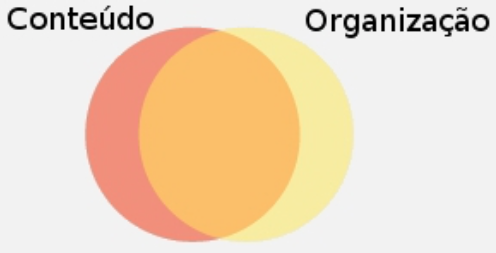
\includegraphics[width=0.7\linewidth]{Figuras/WYSIWYG.png}
    \end{center}
\end{figure}
 
\column{0.5\textwidth}

    \begin{itemize}
    \item Lorem ipsum
    \item Lorem ipsum
    \end{itemize}
    
\end{columns}
     
\end{beamerboxesrounded}

\vfill

\begin{beamerboxesrounded}[upper=fundovermelho,lower=fundocinza,shadow=true]{Lorem ipsum}
   
\begin{columns}
\scriptsize
\column{0.5\textwidth}
\begin{figure}[htb]\label{wysiwym}
    \begin{center}
        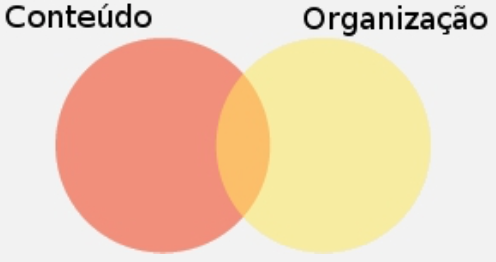
\includegraphics[width=0.7\linewidth]{Figuras/WYSIWYM.png}
    \end{center}
\end{figure}
 
\column{0.5\textwidth}
    \begin{itemize}
    \item Lorem ipsum
    \item Lorem ipsum
    \end{itemize}
\end{columns}
     
\end{beamerboxesrounded}

\end{frame}

%%%%%%%%%%%%%%%%%%%%%%%%%%%%%%%
\subsection[Caixa sem título]{Caixa sem título}
%%%%%%%%%%%%%%%%%%%%%%%%%%%%%%%

%%%%%%%%%%%%%%%%%%%%%%%%%%%%%%%%%%%%%%%%%%%%%%%%%%%%%%
\begin{frame} \frametitle{Caixa sem título}

\begin{beamerboxesrounded}[lower=fundocinza,shadow=true]{}
\begin{itemize}
\item Lorem ipsum
\item \verm{Lorem ipsum}
\item \azul{Lorem ipsum}
\end{itemize}
\end{beamerboxesrounded}

\end{frame}

%%%%%%%%%%%%%%%%%%%%%%%%%%%%%%%
\section[Algoritmo]{Algoritmo}
%%%%%%%%%%%%%%%%%%%%%%%%%%%%%%%

%%%%%%%%%%%%%%%%%%%%%%%%%%%%%%%%%%%%%%%%%%%%%%%%%%%%%%
\begin{frame}[fragile] \frametitle{Algoritmo}

\begin{lstlisting}[language=tex]
\documentclass{article}
\begin{document}
    Exemplo de %Isto é um comentário!!!
        código.
        
    Preste atenção no argumento do begin{frame} desde slide!
    [fragile] é necessário para utilizar o begin{lstlisting}
\end{document}
\end{lstlisting}

\end{frame}

%%%%%%%%%%%%%%%%%%%%%%%%%%%%%%%
\section[Tabela]{Tabela}
%%%%%%%%%%%%%%%%%%%%%%%%%%%%%%%

%%%%%%%%%%%%%%%%%%%%%%%%%%%%%%%%%%%%%%%%%%%%%%%%%%%%%%
\begin{frame} \frametitle{Lorem ipsum}

\begin{beamerboxesrounded}[lower=fundocinza,shadow=true]{}
\begin{table}[]
\begin{tabular}{ccc}
\textbf{Caractere} & \textbf{Significado} & \textbf{Como imprimir} \\ \hline
\textbackslash     & Inicia Comando    & \textbackslash textbackslash         \\
\{ \}              & Agrupamento             & \textbackslash \{  \textbackslash \} \\
\%              & Comentários             & \textbackslash \% \\
\~\   & Espaço indivisível & \textbackslash\~\ \\
\$              & Modo matemático             & \textbackslash \$ \\
\_              & Subscrito/índice             & \textbackslash \_ \\
\^\               & Sobrescrito/expoente             & \textbackslash\^\ \\
\&              & Tabulação             & \textbackslash \& \\
\#              & Ordenação de Parâmetros             & \textbackslash \# \\
\end{tabular}
\end{table}
\end{beamerboxesrounded}

\end{frame}

%%%%%%%%%%%%%%%%%%%%%%%%%%%%%%%
\section[Figura]{Figura}
%%%%%%%%%%%%%%%%%%%%%%%%%%%%%%%

%%%%%%%%%%%%%%%%%%%%%%%%%%%%%%%%%%%%%%%%%%%%%%%%%%%%%%
\begin{frame} \frametitle{Lorem ipsum}
    \begin{figure}[htb]\label{ex1}
        \begin{center}
            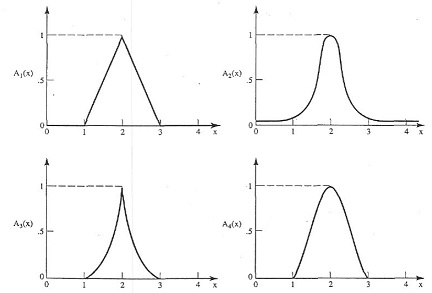
\includegraphics[width=0.75\linewidth]{Figuras/ex1.png}
        \end{center}
        \caption{Exemplo de Figura}
    \end{figure}

\end{frame}

%%%%%%%%%%%%%%%%%%%%%%%%%%%%%%%
\section[Referências]{Referências}
%%%%%%%%%%%%%%%%%%%%%%%%%%%%%%%

%%%%%%%%%%%%%%%%%%%%%%%%%%%%%%%%%%%%%%%%%%%%%%%%%%%%%%
\begin{frame}[allowframebreaks]

    \frametitle{Referências}
    \bibliography{referencias.bib}
        
\end{frame}

\end{document}